\documentclass[11pt]{article}
\usepackage{eadca-template}
\usepackage[plain]{algorithm}

\usepackage[brazil,english]{babel}
\usepackage[utf8]{inputenc}
\usepackage[T1]{fontenc}

\usepackage{graphicx,url}
\usepackage[hang]{subfigure}
\usepackage{psfrag}
\usepackage{amsmath}
\usepackage{amsfonts}
\usepackage{hyperref}

% new packages
\usepackage{enumitem}
\usepackage{balance}
%\usepackage[showframe]{geometry}
%\usepackage{lipsum}
%\usepackage{subfig}
%\usepackage{float}
%\usepackage{subfigure}
%\usepackage{graphicx}
%\usepackage[showframe=true]{geometry}

\sloppy

\title{Using BIC and AIC for Ethernet traffic model selection. Is it worth?}

\author{Anderson dos Santos Paschoalon \and Christian Esteve Rothenberg}

\address{Departamento de Engenharia de Computa\c{c}\~{a}o e Automa\c{c}\~{a}o Industrial (DCA) \\
  Faculdade de Engenharia El\'{e}trica e de Computa\c{c}\~{a}o (FEEC) \\
  Universidade Estadual de Campinas (Unicamp)\\
  Caixa Postal 6101, 13083-970 -- Campinas, SP, Brasil
  \email{\{apaschoalon,chesteve\}@dca.fee.unicamp.br}}

\hyphenation{}
\pagestyle{fancy}

\begin{document}

%%%%%%%%%%%%%%%%%%%%%%%%%%%%%%%%%%%%%%%%%%%%%%%%%%%%%%%%%%%%%%%%%%%%%%%%%%%%%
\twocolumn[
\maketitle
\thispagestyle{fancy}
\selectlanguage{english}

   \begin{abstract}
 In this work, we aim to evaluate how good are the information criterion AIC and BIC inferring which is the best stochastic process to describe Ethernet inter-packet times. Also, we check if there is a practical difference between using AIC or BIC. To do so, we use a set of stochastic distributions to represent inter-packet of a traffic trace and calculate AIC and BIC. To test the quality of  BIC and AIC guesses,  we define a cost function, based on the comparison of significant stochastic properties for internet traffic modeling, such as correlation, fractal-level and mean. Then, we compare both results.  In this short paper, we present just the results of a public free Skype-application packet capture, but we source as reference further analyzes on different traces. We conclude that for most of the cases AIC and BIC can guess right the best fitting, according to the standards of Ethernet traffic modeling. 

   \end{abstract}

  \keywords{BIC, AIC, stochastic function, inter-packet times, correlation, Hurst exponent, heavy-tailed distribution, fractal-level, burstiness, linear-regression, weibull, pareto, exponential, normal, poison, maximum likelihood, Ethernet traffic, traffic modeling, fractal-level, pcap file, Skype traffic}
]

\selectlanguage{English}

\balance
%%%%%%%%%%%%%%%%%%%%%%%%%%%%%%%%%%%%%%%%%%%%%%%%%%%%%%%%%%%%%%%%%%%%%%%%%%%%%%%%
\section{Introduction}\label{sec:introduction}


Emerging technologies such as SDN and NFV are great promises. If succeeding at large-scale, they would change drastically the development and operation of computer networks. But, especially on NFV, its enabling technologies such as virtualization still pose challenges on performance,  reliability, and security\cite{nfv-challenges}. Closed hardware solutions are easier to pass on Service Layer Agreement since they have a much more predictable behavior. Since it is expected virtualization to impact negatively on performance, these VNFs have to keep its degradation as small as possible. Guarantee the Service Layer Agreements on emerging scenarios is now a harder question. There is a demand for more reliable methods to ensure the SLAs, over different types of loads.


It is already a well-known fact that the type of traffic used on performing tests matters. Studies show that a realistic Ethernet traffic provides a different and more variable load characteristics on routers\cite{harpoon-validation}, even with the same mean bandwidth consumption. It indicates that tests with constant bit rate traffic generator tools are not enough for a complete validation of new technologies. There are many reasons for this behavior, which includes burstiness and packet sizes.


A burstier traffic can cause packet more buffer overflows on network \cite{burstiness-queue-lenght} \cite{modelling-of-self-similar} \cite{empirical-interarrival-study}, degenerating network performance\footnote{Fuatures such as packet-trains periods and inter-packet times affect traffic burstiness}, and  measurement accuracy\cite{legotg-paper} \cite{background-traffic-matter}. Another key question is how applications will deal with packets. It is a well-known fact that applications have a huge performance degradation processing small packets\cite{comparative-trafficgen-tools}. A realistic synthetic traffic must not have a single packet-size but must use a distribution \cite{packet-distribution-model}. 


Realistic workload generators are also essential security research\cite{ditg-paper}.  Generation of realistic workloads is important in the evaluation of firewall middleboxes. It includes studies of intrusion, anomaly detection, and malicious workloads\cite{ditg-paper}. 

Since on traditional hardware-based types of \textit{middleboxes}, the impact of realistic traffic is not negligible; we can expect that its impact over virtualized middle-boxes should be even larger, due the extra overhead of a virtualization layer. 


Another critical point is the flow-oriented operation of SDN networks. Each new flow arriving on an SDN switch demands an extra communication load between it and the controller. This may create a bottleneck between the switch and the controller.  Also the SDN switches have a flow-oriented operation. Since its operation relies on queries on flow tables, a stress load must have the same flow properties of an actual Internet Service Provider.


Therefore, there is a demand for the study of the impact of a realistic traffic on this new sort of environment. How VNFs and virtualized middle-boxes and SDN testbeds will behave if stressed with a realistic traffic load in comparison to a constant rate traffic is a relevant subject. 


%%%%%%%%%%%%%%%%%%%%%%%%%%%%%%%%%%%%%%%%%%%%%%%%%%%%%%%%%%%%%%%%%%%%%%%%%%%%%%%%
\section{Open-source Solutions}\label{sec:review}


The open-source community offers a huge variety of workload generators and benchmarking tools \cite{ditg-paper}\cite{validate-trafficgen}\cite{comparative-trafficgen-tools}\cite{performance-trafficgen}. Most of these tools were built for specific purposes and goals, so each uses different methods of traffic generation, and enable controll of different features, such as throughput (bits/bytes per second, packets per seconds), packet-sizes, protocols and header customization, payload customization, inter-packet times, On/Off periodos, start and sending time, and emulation of applications such as Web server/client communication, VoIP, HTTP, FTP, p2p applications, and many more.


Some traffic generator tools offer support emulation of single application workloads. But this does not correspond to real complex scenarios. Other tools work as packet replay engines, such as TCPreplay and TCPivo. Although in that way is possible to produce a realistic workload at high rates, it comes with some issues. First, the storage space required becomes huge for long-term and high-speed traffic capture traces. Also, obtaining good traffic traces sometimes is hard, due privacy issues and fewer good sources. 


Many tools support a larger set of protocols and high-performance, such Seagull and Ostinato. Others are also able to control inter-packet times and packet sizes using stochastic models, like D-ITG\cite{ditg-paper} and MoonGen. But all of them just offer a complet framework to be congfigured, but the customization of the traffic is all up to user to do. So, there is no simple way for the user to create an synthetic realistic traffic scenario. 

We also have available a variety of APIs that enable creation of traffic and custom packets, wich include low-level APIs, such as Linux Socket API,  Libpcap, Libtins, DPDK, Pcapplusplus, libcrafter, impacket, scapy and many others. These APIs enable a finer controll and customization over each packet, and are used to implement traffic generators. For example, Ostinato and TCPreplay uses Libpcap, and MoonGen uses DPDK. Also, many of the listed traffic generators provides their own API, such as Ostinato Python API, D-ITG C API, and MoonGen LUA API. 


%They can give a good control of the traffic and high rates. Es example of controllable features we can list:
%\begin{itemize}
%\item Throughput, the number of bytes, number of packets.
%\item Protocols. Most of the tools give support to network and transport protocols. Many also offer support to Link and Application protocols;
%\item Header and payload configuration. Support for header customization includes source and destination port/addresses, QoS parameters, flags, etc. Some traffic generators also allow customizing payload bytes.
%\item Inter-packet times. Some tools offer a set of stochastic distributions to control inter-packet times. The user can use these stochastic functions to emulate realistic inter-arrival times.
%\item On/off periods: support of packet trains periods. Many offer stochastic models to control it. 
%\item Sending time and start-time: the user can use these features to control flows timings.  
%\item Packet-size: support for different packet sizes. Some tools offer constant values or stochastic distributions to control packet sizes.
%\item Paralell flows configuration.
%\item Emulation of specific applications: common examples are 
%\end{itemize}


Therefore we have a large variety open-source tools available for custom traffic generation. But reproducing a realistic traffic scenario is a hard question. Selecting the right framework, a good traffic model, and the right configuration, is by itself a complex research project\cite{legotg-paper}\cite{selfsimilar-ethernet}. But usually this is not the goal of the project, so the researcher or the them have scarce time available to work over it. Since it is usually is not the main goal of the project, but just a mean many times a simplistic and irrealistic sollution is opt because of the limited resources such as time and manpower.   Reproducig a realistic traffic usung these tools is a manual process and demands implementation of scripts or programs leveraging human (and scarce) expertise on network traffic characteristics  and experimental evaluation. Since it usually is not the goal of the research, but a mean. 


For this gap, there are some sollutions on the open source community. Tools like Swing and Harpoon uses capture traces to set intern parameters, enabling an easier configuration. Also, Swing uses complex multi-levels models which are able to provide a high degree of realism\cite{swing-paper}. But they have their issues as well. Harpoon does not configure parameters at packet level\cite{harpoon-paper} and is not supported by newer Linux kernels, what may be a huge problem with setup and configuration. Swing\cite{swing-paper} aims to generate realistic traffic, but focous on background traffic, and high throughputs it is not a goal off the application\cite{swing-paper} \cite{legotg-paper}. Due the fact that its traffic generation engine is coupled to its modeling framework, you can't opt to use a newer/faster packet generation library. The only way of replacing the traffic engine is changing and recompiling the original code. This is clearly a hard task\cite{legotg-paper}, and an error prone activity. Again, we fall in the same problem a complex task that usually is not the goal of the project. 

Another issue is the large variety of tools, and different methods of configuration and limitations. To create a custom traffic, a user must read large manuals, and custom-design scripts. One of our bigger proposals is create a tool able to automatically do this processes. So The user may design his custom traffic by creating his own Compact Trace Descriptor, and create a traffic using many different tools, like Ostinato, D-ITG, Iperf, but not caring about how to proper configure each of them. 


%Since synthetic traffic traces generation is mature in academia, the creation of custom network workloads through the configuration of  open-source tools is an affordable task. But it is not often available in an automatic way, and most of the times is a challenging question\cite{legotg-paper}, and still, requires expert knowledge. It requires time, study, and is vulnerable to human mistakes and lack of validation. Such work may require weeks to complete a realistic reproduction of a single scenario, so most of the time it is just not done. We argue that widely (i.e. affordable) existing approaches can be regarded as simplistic often point solutions to more general cases. 


% Also, just choosing which workload generator tool may fit better for the user needs is not a simple question. Tools like D-ITG\footnote{\href{http://traffic.comics.unina.it/software/ITG/}{http://traffic.comics.unina.it/software/ITG/}} provide support to many different stochastic functions, Ostinato\footnote{\href{http://ostinato.org/}{http://ostinato.org/}} provides a larger support for protocols, and a higher throughput for each thread\cite{comparative-trafficgen-tools}, and others like Seagull\footnote{\href{http://gull.sourceforge.net/doc/WP_Seagull_Open_Source_tool_for_IMS_testing.pdf}{http://gull.sourceforge.net/doc/WP\_Seagull\_Open\_Source\_tool\_for\_IMS\_testing.pdf}} are responsive. 



%%%%%%%%%%%%%%%%%%%%%%%%%%%%%%%%%%%%%%%%%%%%%%%%%%%%%%%%%%%%%%%%%%%%%%%%%%%%%%%%%%%%%%%%%%%%%%%%%%%%%%%%%%
\section{Architecture and Modelling}\label{sec:architecture}

To meet the requirements presented in the section ~\ref{sec:introduction}, we will define our solution, and how it works. SIMITAR architecture is presented in the figure~\ref{fig:architecture}. It is composed of four components: a \textit{Sniffer}, a \textit{SQLite database}, a \textit{TraceAnalyzer}, a \textit{FlowGenerator};  and a \textit{Network Traffic Generator}, as subsystem. We describe each part below.

\begin{figure}[ht!]
        \centering
        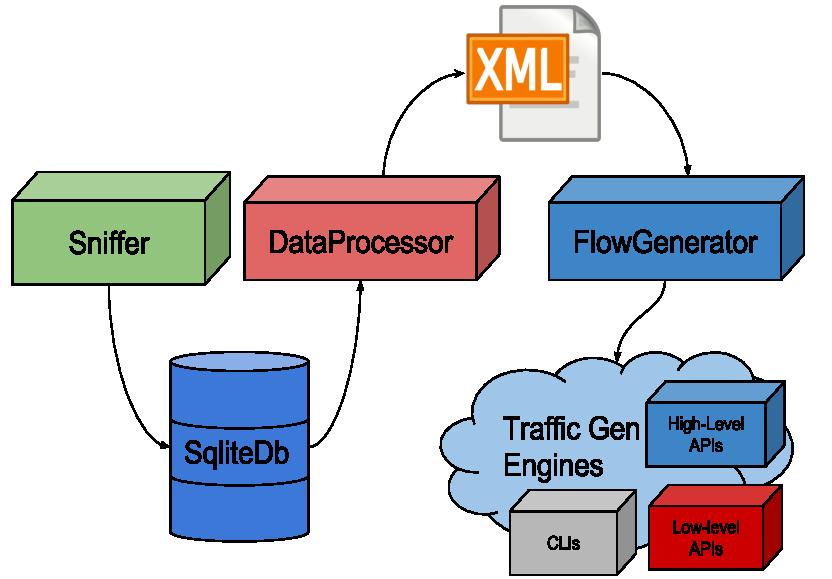
\includegraphics[height=2.7in]{figures/architecture-diagram}
        \caption{Architecture of SIMITAR}
    \label{fig:architecture}
\end{figure}


%%%%%%%%%%%%%%%%%%%%%%%%%%%%%%%%%%%%%%%%%%%%%%%%%%%%%%%%%%%%%%%%%%%%%%%%%%%%%%%%
\subsection{Sniffer}


This component collects network traffic data and classifies it into flows, storing stores in an SQLite database. It defines each flow by the same criteria used by SDN switches\cite{sdn-survey},  through header fields matches. It uses:

\begin{itemize}
\item Link Protocol
\item Network Protocol
\item Network Source and Destination Address
\item Transport Protocol
\item Transport Source and Destination Port
\end{itemize}

\begin{figure}[ht!]
        \centering
        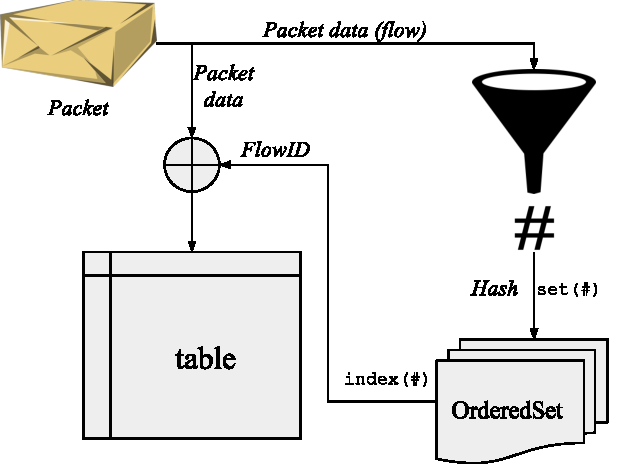
\includegraphics[width=\linewidth]{figures/sniffer-classifier}
        \caption{SIMITAR's sniffer hash-based flow classification}
    \label{fig:sniffer}
\end{figure}
 
It has a data structure we developed called \textit{OrderedSet}. A set is a list of elements with no repetition but does not keep track of the insertion order. Our OrderedSet does. Also, it makes use of a  64 bits hash function of the family FNV\footnote{The collision probability of a good 64 bits hash function in a table with 10000 items is about of $2.71e-12$.}. The listed header fields are inputs for a hash function, and its value is set on the ordered set which returns its order (index on the \textit{OrderedSet}). The index value is chosen as a packet flowID.

%%%%%%%%%%%%%%%%%%%%%%%%%%%%%%%%%%%%%%%%%%%%%%%%%%%%%%%%%%%%%%%%%%%%%%%%%%%%%%%%
\subsection{SQLite database}

\begin{figure}[ht!]
        \centering
        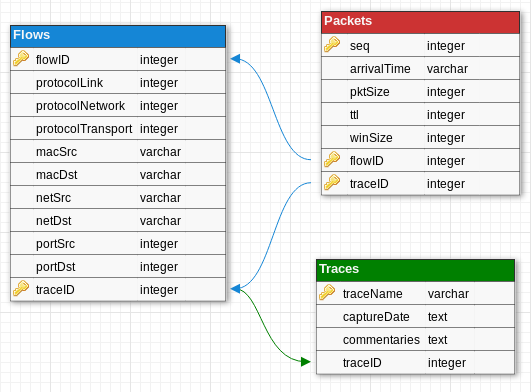
\includegraphics[width=\linewidth]{figures/database-relational-model}
        \caption{SIMITAR's SQLite database relational model}
    \label{fig:simitar-database}
\end{figure}


The database stores the collected raw data from the traces for further analysis. The \textit{Sniffer} and the \textit{TraceAnalyzer} components uses the database.  We choose an SQLite database, because according to its specifications\footnote{\href{https://www.sqlite.org/whentouse.html}{https://www.sqlite.org/whentouse.html}}, it fits well our purposes. It is simple and well-suitable for an amount of data smaller than terabytes. In the figure ~\ref{fig:simitar-database} we present the relational model of our database, which stores a set of features extracted from packets, along with the flowID calculated by the sniffer component. 


%%%%%%%%%%%%%%%%%%%%%%%%%%%%%%%%%%%%%%%%%%%%%%%%%%%%%%%%%%%%%%%%%%%%%%%%%%%%%%%%%%%%%%%%%%%%%%%%%%%%%%%%%%
\subsection{Trace Analyzer}


This module is the core of our project. It creates a trace model via the analysis of the collected data. We define here a Compact Trace Descriptor (CTD) as a human and machine-readable file, which describes a traffic trace through a set of flows, each of them represented by a set of parameters, such as header information and analytical models.  The Trace Analyze has the task to learn these features from raw traces data (stored in the SQLite database) and generate an XML file.  In the figure~\ref{fig:CTD-diagram} we show a directory diagram of a CDT file. It has many of many flow fields, and each one contains each parameter estimated. Now we will describe how we construct it. 

\begin{figure}[ht!]
        \centering
        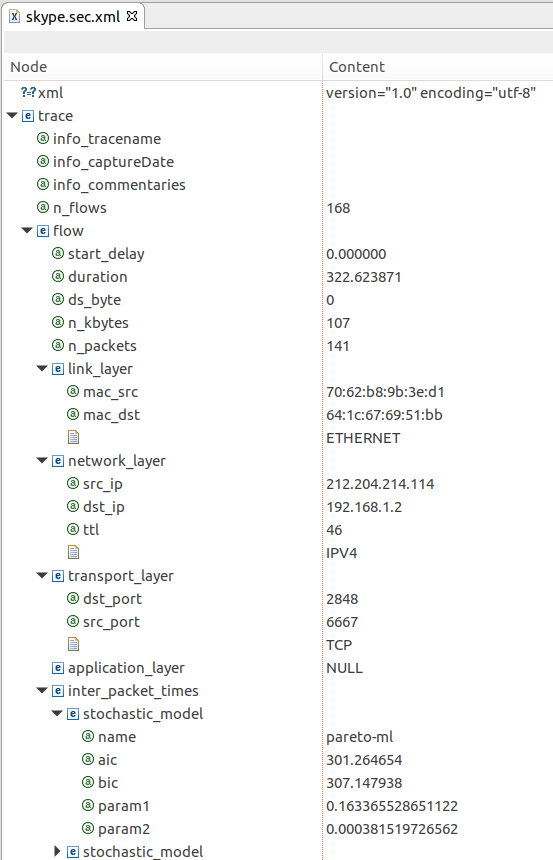
\includegraphics[width=\linewidth]{figures/cdt1}
        \caption{Directory diagram of the schema of a Compact Trace Descriptor (CDT) file.}
    \label{fig:CTD-diagram}
\end{figure}

\subsubsection{Flow features}

Some unique per-flow features are directly measured from the data. They are:  

\begin{itemize}
\item Flow-level properties like duration of flow, start delay, number of packets per flow, number of KBytes per flow; 
\item Header fields, like protocols, QoS fields, ports, and addresses.
\end{itemize}

Each one of these parameters is unique per flow. Other features like PSD (packet size distribution) e IPT (Inter-packet time), have a more complex behavior.  To represent these characteristics, we will use sets of stochastic-based models.  


\subsubsection{Inter Packet Times}

To represent inter-packet times, we adopt a simplified version of the Harpoon's traffic model. A deep explanation of the original model can be found at \cite{harpoon-paper} and \cite{harpoon-validation}. Here, we will explain our simplified version, which is illustrated at figure~\ref{fig:modified-harpoon-model}. 

Harpoon uses a definition of each level, based on the measurement of SYN and ACK TCP flags. It uses TCP flags (SYN) to classify packets in different levels, named their file, session, and user level. We choose to estimate these values, based on inter-packet times only. The distinction is made based on the time delay between packets.


In our algorithm simplified version, we define three different layers of data transference to model and control: file, session, and flow. For SIMITAR, a file is just a sequence of consecutive packets transmitted continuously, without large interruption of traffic. It can be, for example, packets sent downloading a file, packets from a  UDP  connection or a single ICMP echo packet. The session-layer refers to a sequence of multiple files transmitted between a source and a destination, belonging to the same flow.  The flow level refers to the conjunct of flows, as classified by the Sniffer.  Now, we explain SIMITAR operation on each layer. 


In the \textbf{flow layer} the \textit{TraceAnalyzer} loads the flow arrival times from the database and calculates the inter-packet times within the flow context. 


At the \textbf{session layer}, we use a deterministic approach for evaluating file transference time and times between files: ON/OFF times sequence of packet trains. We choose a deterministic model because in this way we can express diurnal behavior\cite{harpoon-paper}.  We develop an algorithm called \textit{calcOnOff} responsible for estimating these times. It also determines the number of packets and bytes transferred by each file. Since the ON times will serve as input for actual traffic generators, we defined a minimum acceptable time for on periods equals to 100 ms. ON times can be arbitrary smalls, and they could be incompatible with acceptable ON periods for traffic generators. Also in the case of just one packet, the ON time would be zero. So setting a minimum acceptable time to solve these issues. The OFF times, on the other hand, are defined by the constant \texttt{session\_cut\_time} \footnote{In the code it is called \texttt{DataProcessor::m\_session\_cut\_time} }. If the time between two packets of the same flow is larger than \texttt{session\_cut\_time}, we consider them belonging to a different file, so this time is a session OFF time. In this case, we use the same value of the constant \textit{Request and Response timeout} of Swing\cite{swing-paper} for the \texttt{session\_cut\_time}: 30 seconds. The control of ON/OFF periods in the traffic generation is made by the \textit{Flow Generator} component \footnote{This control is made by the class \texttt{NetworkFlow}}.


In the \textbf{file layer}, we model the inter-packet times at the file level. To estimate inter-packet times within files, we select all inter-packet times smaller than \texttt{session\_cut\_time}\footnote{In the code it is called\texttt{DataProcessor::m\_session\_cut\_time} }. All files within the same flow are considered to follow the same model. We delegate the control of the inter-packet times to the underlying workload engine tool. We ordered them, from the best to the worst. Currently, we are using eight different stochastic functions parameterizations. They are Weibull(linear regression), Normal(mean/standard deviation calculation), Exponential(mean and linear regression estimation), Pareto(linear regression and maximum likelihood), Cauchy(linear regression) and Constant(mean calculation). From those, Weibull, Pareto, and Cauchy are heavy-tailed functions, and therefore self-similar processes. But if the flow has less than 30 packets, just the constant model is evaluated. It is because numerical methods gave poor results if the data sample used is small. We sort these models according to the Akaike Information Criterion (AIC) as default\cite{sourcesonoff-paper}\cite{bic-aic-comparision}. We will enter into deeper details on this methodology on the chapter ~\ref{ch:modeling-evaluation}. The methodology of selection is presented in the figure~\ref{fig:model-parameterization}, and all constants and modes of operation can be changed by command line options.


\subsubsection{Packet Sizes}


Our approach for the packet size is much simpler. Since the majority of packet size distribution found on real measurements are bi-modal \cite{packet-distribution-model}\cite{sourcesonoff-paper}\cite{udp-flows-model}, we first sort all packet sizes of flow in two modes. We define a packet size mode cut value of 750 bytes, same value adopted by \cite{udp-flows-model}. 


We know how much packets each mode has, and then we fit a model for it. We use three stochastic models: constant, exponential and normal. Since self-similarity does not make sense for packet-sizes, we prefer to use just the simpler models. When there is no packet for a model, we set a flag NO\_MODEL, and when there is just a single packet we just use the constant model. Then calculate the BIC and AIC for each, but we decide to set the constant model as the first.

As is possible to see in many works \cite{packet-distribution-model} \cite{udp-flows-model}, since the standard deviation of each mode tends to be small, constant fittings use to give good approximations. Also, it is computationally cheaper for the traffic generated than the other models, since no calculation is a need for each packet sent. Since both AIC and BIC criteria always will select the constant model as the worst, we decide to ignore this.

\subsubsection{Packet Sizes}

Our approach for the packet size is much simpler. Since the majority of packet size distribution found on real measurements are bi-modal \cite{packet-distribution-model}\cite{sourcesonoff-paper}\cite{udp-flows-model}, we first sort all packet sizes of flow in two modes. We define a packet size mode cut value of 750 bytes, same value adopted by \cite{udp-flows-model}. 

We know how much packets each mode has, and then we fit a model for it. We use three stochastic models: constant, exponential and normal. Since self-similarity does not make sense for packet-sizes, we prefer to use just the simpler models. When there is no packet for a model, we set a flag NO\_MODEL, and when there is just a single packet we just use the constant model. Then calculate the BIC and AIC for each, but we decide to set the constant model as the first.

As is possible to see in many works \cite{packet-distribution-model} \cite{udp-flows-model}, since the standard deviation of each mode tends to be small, constant fittings use to give good approximations. Also, it is computationally cheaper for the traffic generated than the other models, since no calculation is a need for each packet sent. Since both AIC and BIC criteria always will select the constant model as the worst, we decide to ignore this.


%%%%%%%%%%%%%%%%%%%%%%%%%%%%%%%%%%%%%%%%%%%%%%%%%%%%%%%%%%%%%%%%%%%%%%%%%%%%%%%%%%%%%%%%%%%%%%%%%%%%%%%%%%
\section{Validation}\label{sec:validation}


\subsection{Methodology}

As proof of concepts for our tool, we are going to use Mininet's emulated testbeds. We automate all tests using scripts, so our experiments are are fully  reproducible. They are responsible for running all the proposed tests in this chapter and perform the calculations. It includes:

\begin{itemize}
	\item Build the topology;
	\item Run the SIMITAR traffic generator;
	\item Collect the packeckets as \textit{pcap} files, and stract data from it;
	\item Perform the proposed proof of concept analysis;
	\item Plot the data.
\end{itemize}

Each test is organized as a Python packege, responsible for tigger all the applications and procedures. The parameters for each simulation can be configured by a \textit{config.py} file. The files \textit{README} on each packege, provide a tutorial to run correctely each test. With all tools instaled, less then fifteen minutes is enought for run each test again. A complete specification of our scenario we show at the table ~\ref{tab:specifications}, including the hardware specificatins and the software versions. 

\begin{table}[ht!]
	\centering
	\caption{Experiments specification table}
	\label{tab:specifications}
	\begin{tabular}{ll}
		\hline
		Processor            & Intel(R) Core(TM) i7-4770, 8 cores, CPU @ 3.40GHz \\
		RAM                  & 15.5 GB                                           \\
		HD                   & 1000 GB                                           \\
		Linux         & 4.8.0-59-generic                                  \\
		Ubuntu        & Ubuntu 16.10 (yakkety)                            \\
		SIMITAR       & v0.4.2 (Eulemur rubriventer)                      \\
		Mininet       & 2.3.0d1                                           \\
		Iperf         & iperf version 2.0.9 (1 June 2016) pthreads        \\
		Libtins       & 3.4-2                                             \\
		OpenDayLight  & 0.4.0-Beryllium                                   \\
		Octave        & 4.0.3                                             \\
		Pyshark       & 0.3.6.2                                     \\
		Wireshark     & 2.2.6+g32dac6a-2ubuntu0.16.10               \\
		Tcudump       & 4.9.0 \\
		libpcap       & 1.7.4\\
		\hline
	\end{tabular}
\end{table}


\begin{figure}[h!]
	\centering
	\subfloat[Single hop SDN topology]{
		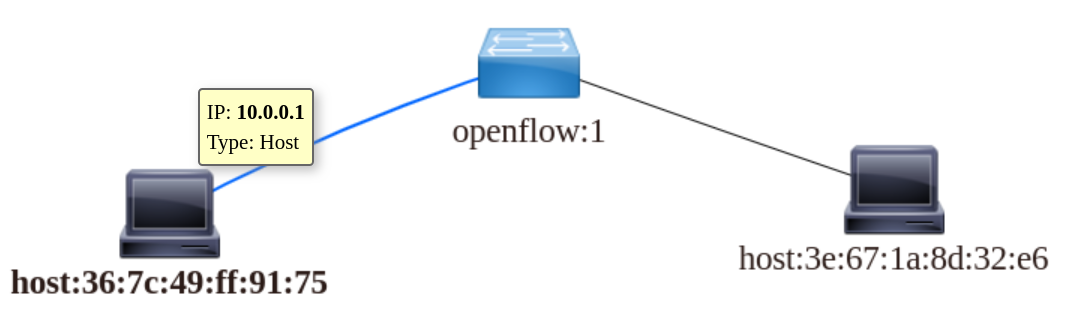
\includegraphics[width=\linewidth]{figures/topo-simple}
		\label{fig:topo-simple}
	}
	\hspace{0mm}
	\subfloat[Tree SDN topology]{
		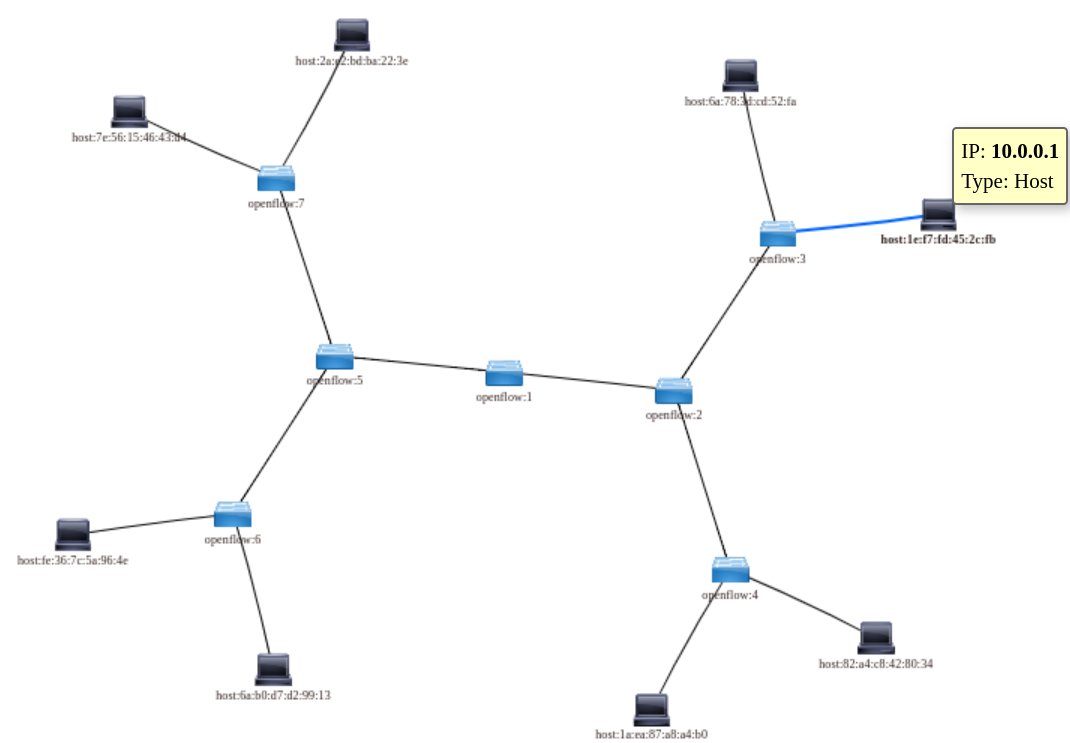
\includegraphics[width=\linewidth]{figures/topo-tree}
		\label{fig:topo-tree}
	}
	\hspace{0mm}
	\caption{Mininet SDN topologies. Controller OpenDayLight Beryllium.)}
	\label{fig:topo}
\end{figure}


For each test, we generate a set of plots to compare the original and synthetic trace. Two of them we use for mere visual comparison: flows per second and bandwidth. To compare the realism quality of the generated traffic, we plot the flows cumulative distribution function (CDF)\cite{harpoon-paper}, and the Wavelet multiresolution analysis.  On every case, the more closer the plots are, the more similar the traffics are according to each perspective. Also, we wrote in the table ~\ref{tab:results-summary} a complation of each traffic statistics. 

The flow's cumulative distribution measures each new flow identified the trace. It is a measure similarity of the traffic at the flow-level.  The wavelet multiresolution analysis is capable of capture traffic scaling characteristics and is a measure of similarity at the packet-level. If the value decreases, a periodicity on that time scale exists. With white-noise features, the traffic will remain constant. If the traffic has self-similar characteristics on a particular time scale, its value will increase linearly.

We use as testbeds: a tree topology (figure~\ref{fig:topo-tree}), similar to tests performed by Swing\cite{swing-paper}\cite{background-traffic-matter}\cite{legotg-paper}, and a one-hop connection of two hosts. Both topologies are SDN networks and have OpenDayLight Beryllium as the controller.

For generating the traffic on the host \textit{h1} with IPv4 address 10.0.0.1. The traffic is captured from the host interface with TCPdump in a \textit{pcap} format.  We organized the project directory tree as follows\footnote{ \href{https://github.com/AndersonPaschoalon/ProjetoMestrado}{https://github.com/AndersonPaschoalon/ProjetoMestrado} }: the software is at \textit{SIMITAR}. All validation tests and project prototypes we aved at \textit{Tests} directory. The software documentation is at \textit{Docs} directory.

We use SIMITAR v0.4.2 (Eulemur rubriventer)\footnote{ We label the tags of SIMITAR control version on GitHub as lemurs species names (\href{https://en.wikipedia.org/wiki/List_of_lemur_species}{https://en.wikipedia.org/wiki/List\_of\_lemur\_species})}, as tagged at the GitHub repository.  SIMITAR already have two functional traffic generator engines: Iperf and libtins C++ API.  


\begin{table*}[h]
	\centering
	\caption{Sumary of results comparing the original traces (italic) and te traffic generated by SIMITAR, with the description of the scenario.}
	\label{tab:results-summary}
	%\scalebox{0.87}{
\begin{tabular}{lcccccc}
	\hline
	\multicolumn{1}{c}{\multirow{3}{*}{}} & \multirow{3}{*}{\textit{skype-pcap}} & \multicolumn{1}{c}{\multirow{3}{*}{\begin{tabular}[c]{@{}c@{}}skype, \\ one-hop, \\ iperf\end{tabular}}} & \multicolumn{1}{c}{\multirow{3}{*}{\begin{tabular}[c]{@{}c@{}}skype, \\ tree, \\ iperf\end{tabular}}} & \multicolumn{1}{c}{\multirow{3}{*}{\begin{tabular}[c]{@{}c@{}}skype, \\ one-hop, \\ libtins\end{tabular}}} & \multirow{3}{*}{\textit{lgw10s-pcap}} & \multicolumn{1}{c}{\multirow{3}{*}{\begin{tabular}[c]{@{}c@{}}lgw10s, \\ one-hop, \\ libtins\end{tabular}}} \\
	\multicolumn{1}{c}{}                  &                             & \multicolumn{1}{c}{}                                                                                     & \multicolumn{1}{c}{}                                                                                  & \multicolumn{1}{c}{}                                                                                       &                              & \multicolumn{1}{c}{}                                                                                        \\
	\multicolumn{1}{c}{}                  &                             & \multicolumn{1}{c}{}                                                                                     & \multicolumn{1}{c}{}                                                                                  & \multicolumn{1}{c}{}                                                                                       &                              & \multicolumn{1}{c}{}                                                                                        \\ \hline
	Hurst Exponent                        & 0.601                       & 0.618                                                                                                    & 0.598                                                                                                 & 0.691                                                                                                      & 0.723                        & 0.738                                                                                                       \\
	Data bit rate (kbps)                  & 7                           & 19                                                                                                       & 19                                                                                                    & 12                                                                                                         & 7252                         & 6790                                                                                                        \\
	Average packet rate (packets/s)       & 3                           & 4                                                                                                        & 5                                                                                                     & 6                                                                                                          & 2483                         & 2440                                                                                                        \\
	Average packet size (bytes)           & 260,89                      & 549,05                                                                                                   & 481,14                                                                                                & 224,68                                                                                                     & 365,00                       & 347,85                                                                                                      \\
	Number of packets                     & 1071                        & 1428                                                                                                     & 1604                                                                                                  & 2127                                                                                                       & 24 k                         & 24 k                                                                                                        \\
	Number of flows                       & 167                         & 350                                                                                                      & 325                                                                                                   & 162                                                                                                        & 3350                         & 3264                                                                                                        \\ \hline
\end{tabular}
	%}
\end{table*}

For schedule of the timing of traffic generated by each flow, we implemented three methodologies: \texttt{usleep()} C function,\texttt{select()} C function and \textit{pooling}. Here we use \texttt{usleep()} . We implemented the class \texttt{IperfFlow,} responsible for generate the traffic of each flow, using \texttt{popen()} and \texttt{pclose()} to instantiate Iperf processes, responsible for generating the traffic. Traffic customization on Iperf has many limitations. It cannot assign arbitrary IP addresses as source and destination since it must establish a connection between the source and destination. For the transport layer, it just supports TCP and UDP protocol, and constant bandwidth traffic. On the other hand, it enables customization of transmission time, number of packets, windows size, TTL, packet sizes, payload and many other features. Since Iperf has to establish a communication, SIMITAR must operate in the client mode on the source, and server mode on the destinations.

Libtins enable the creation and emission of arbitrary packets and do not require the establishment of a connection.  Thus SIMITAR does not need to operate in server mode on the destination. The packet customization capability is vast, and enable a full usage of our model parameters. Control inter-packet times stays for future work. 

\subsection{Results}



% Bandwidth
\begin{figure}[h!]
	\centering
	\subfloat[\textit{Iperf, single-hop, skype-pcap}]{
		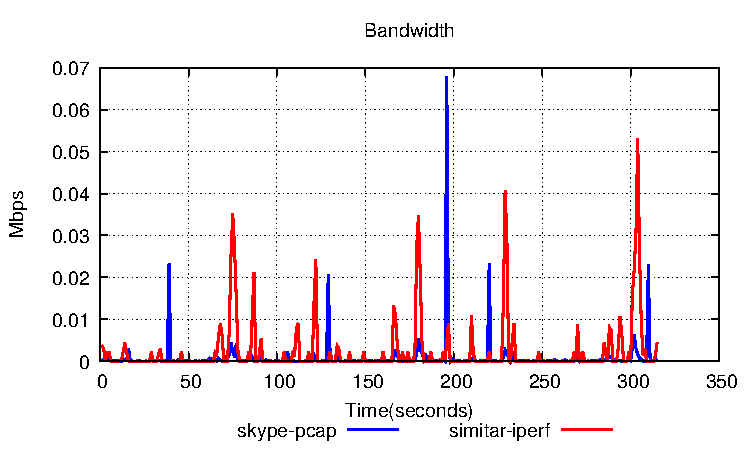
\includegraphics[width=77mm]{figures/skype-iperf-Bandwidth.pdf}
		\label{fig:iperfBw}
	}
	\hspace{0mm}
	\subfloat[\textit{Iperf, tree, skype-pcap}]{
		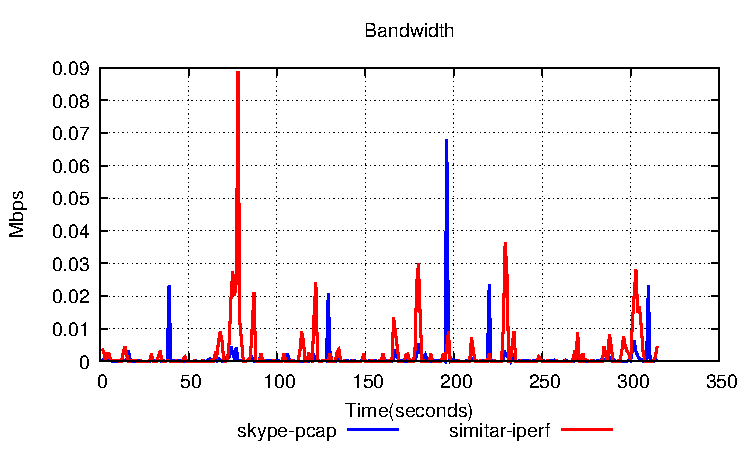
\includegraphics[width=77mm]{figures/skype-tree-iperf-Bandwidth.pdf}
		\label{fig:iperftreeBw}
	}
	\hspace{0mm}
	\subfloat[\textit{libtins, single-hop, skype-pcap}]{
		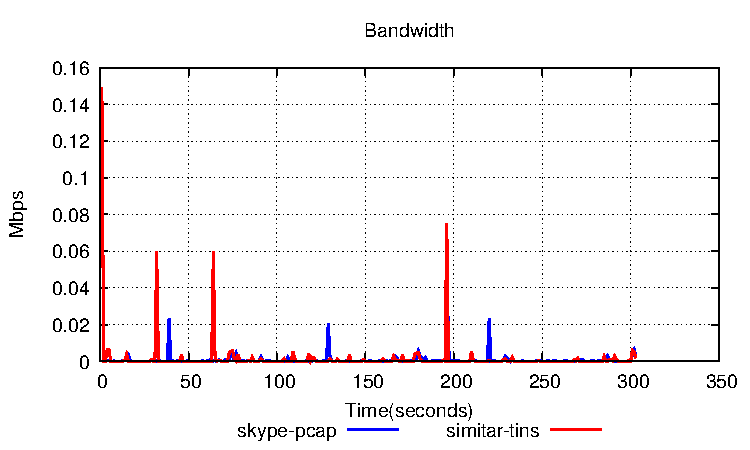
\includegraphics[width=77mm]{figures/skype-tins-Bandwidth.pdf}
		\label{fig:tinsBw}
	}
	\hspace{0mm}
	\subfloat[\textit{libtins, single-hop, langw10s-pcap}]{
		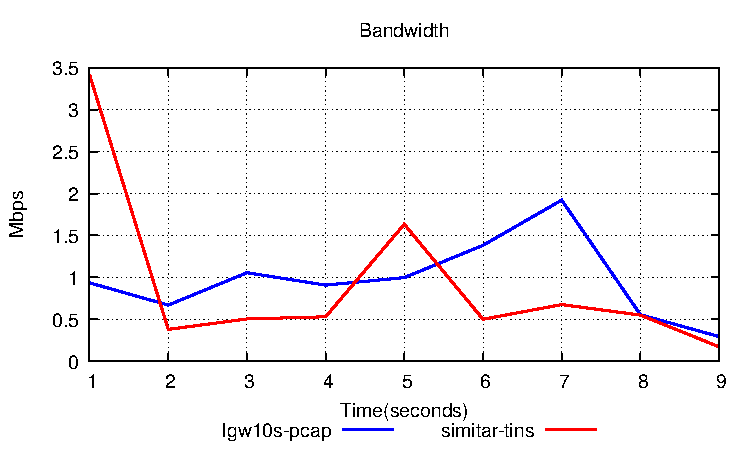
\includegraphics[width=77mm]{figures/lgw-tins-Bandwidth.pdf}
		\label{fig:tinsLgwBw}
	}
	\hspace{0mm}
	\caption{Traces bandwidth.}
	\label{fig:flows-bandwidth}
\end{figure}
% Flows per second
\begin{figure}[ht!]
	\centering
	\subfloat[\textit{Iperf, single-hop, skype-pcap}]{
		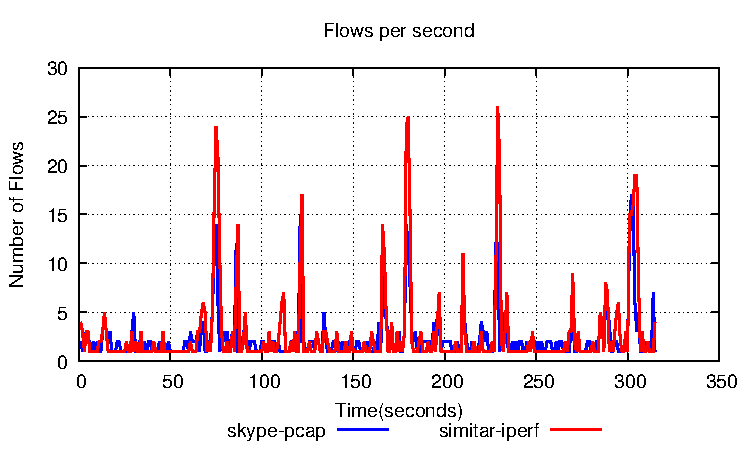
\includegraphics[width=77mm]{figures/skype-iperf-FlowsPs.pdf}
		\label{fig:iperfFps}
	}
	\hspace{0mm}
	\subfloat[\textit{Iperf, tree, skype-pcap}]{
		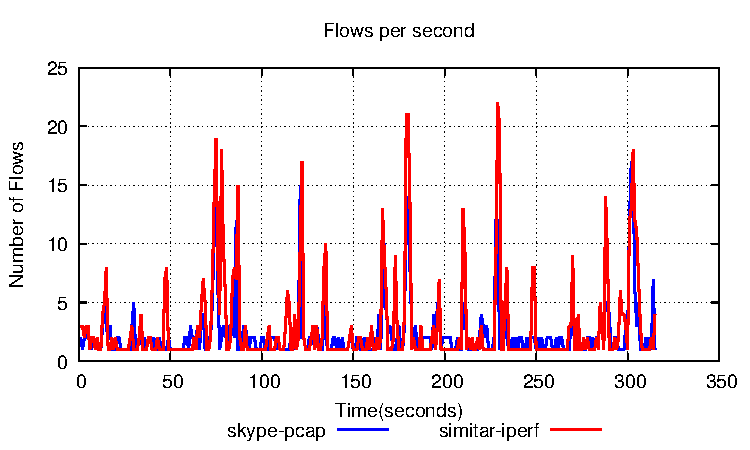
\includegraphics[width=77mm]{figures/skype-tree-iperf-FlowsPs.pdf}
		\label{fig:iperftreeFps}
	}
	\hspace{0mm}
	\subfloat[\textit{libtins, single-hop, skype-pcap}]{
		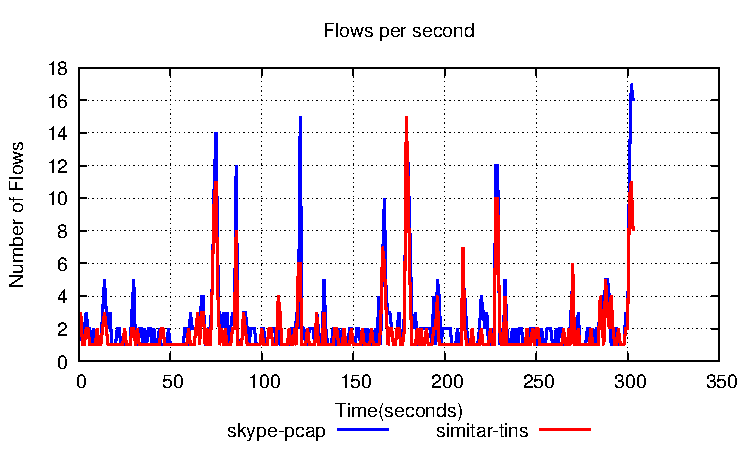
\includegraphics[width=77mm]{figures/skype-tins-FlowsPs.pdf}
		\label{fig:tinsCdf}
	}
	\hspace{0mm}
	\subfloat[\textit{libtins, single-hop, langw10s-pcap}]{
		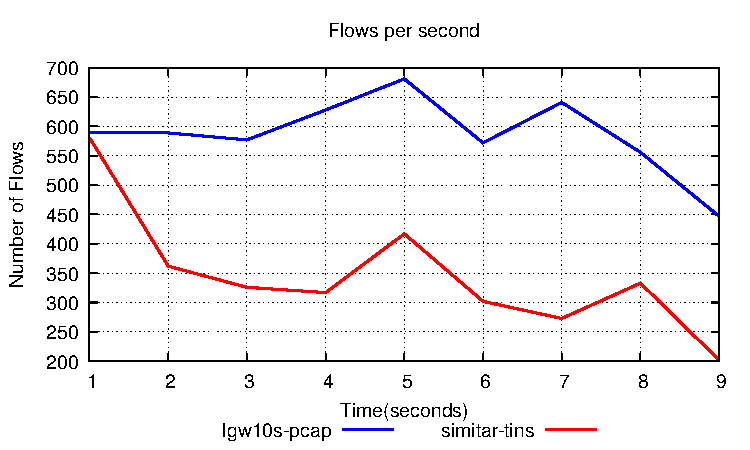
\includegraphics[width=77mm]{figures/lgw-tins-FlowsPs.pdf}
		\label{fig:tinsLgwFps}
	}
	\hspace{0mm}
	\caption{Flow per seconds}
	\label{fig:flows-ps}
\end{figure}
% Flow CDF
\begin{figure}[ht!]
	\centering
	\subfloat[\textit{Iperf, single-hop, skype-pcap}]{
		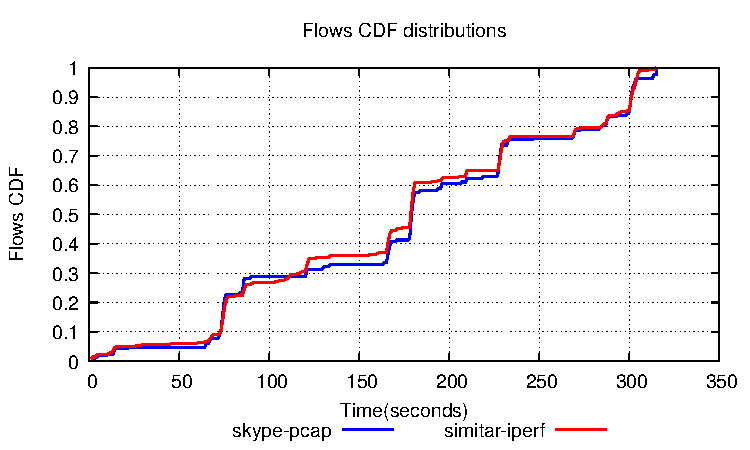
\includegraphics[width=77mm]{figures/skype-iperf-FlowCdf.pdf}
		\label{fig:iperfCdf}
	}
	\hspace{0mm}
	\subfloat[\textit{Iperf, tree, skype-pcap}]{
		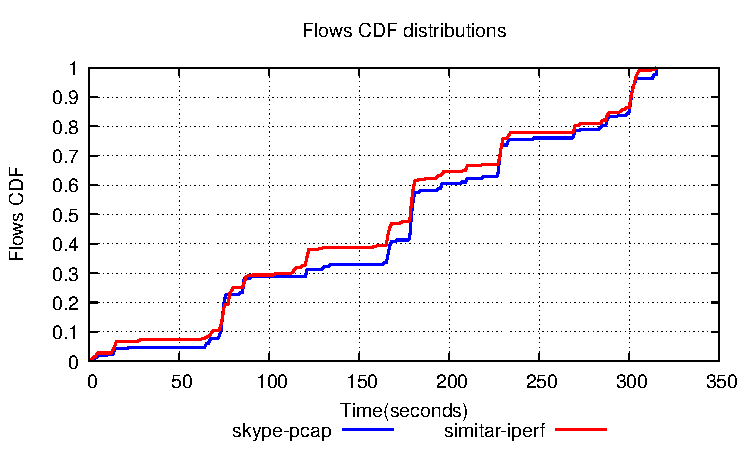
\includegraphics[width=77mm]{figures/skype-tree-iperf-FlowCdf.pdf}
		\label{fig:iperftreeCdf}
	}
	\hspace{0mm}
	\subfloat[\textit{libtins, single-hop, skype-pcap}]{
		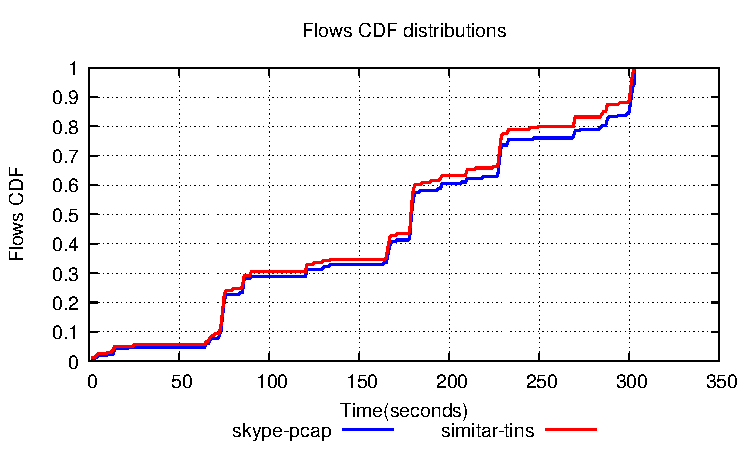
\includegraphics[width=77mm]{figures/skype-tins-FlowCdf.pdf}
		\label{fig:tinsCdf}
	}
	\hspace{0mm}
	\subfloat[\textit{libtins, single-hop, langw10s-pcap}]{
		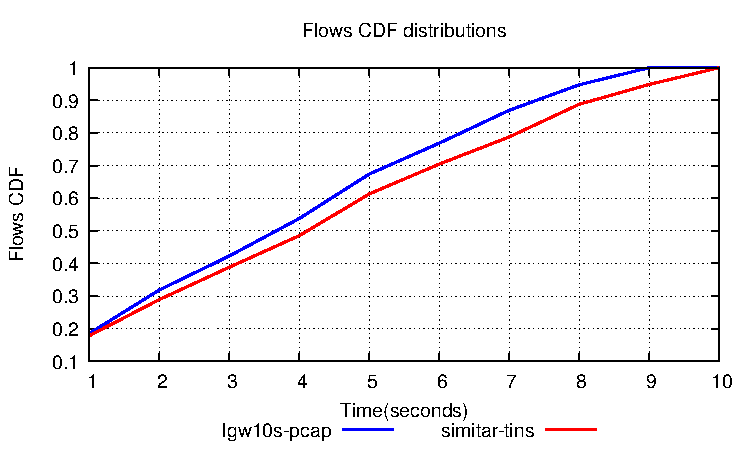
\includegraphics[width=77mm]{figures/lgw-tins-FlowCdf.pdf}
		\label{fig:tinsLgwCdf}
	}
	\hspace{0mm}
	\caption{Flows cumulative distributions.}
	\label{fig:flows-cdf}
\end{figure}
% Wabelet
\begin{figure}[h!]
	\centering
	\subfloat[\textit{Iperf, single-hop, skype-pcap}]{
		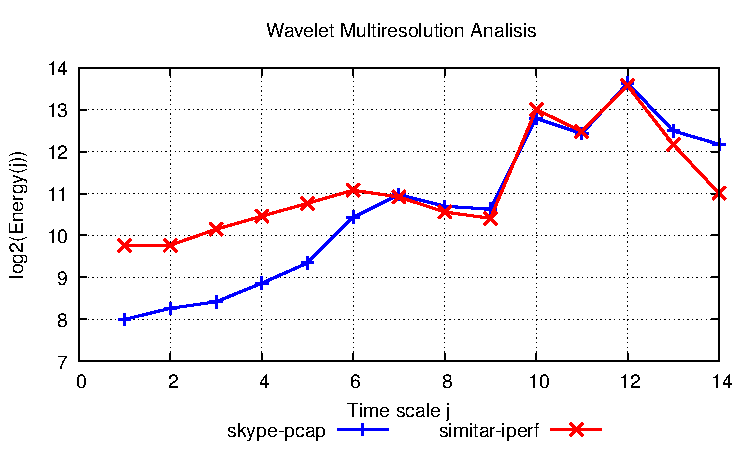
\includegraphics[width=77mm]{figures/skype-iperf-WaveletMREA.pdf}
		\label{fig:iperfWaveletMREA}
	}
	\hspace{0mm}
	\subfloat[\textit{Iperf, tree, skype-pcap}]{
		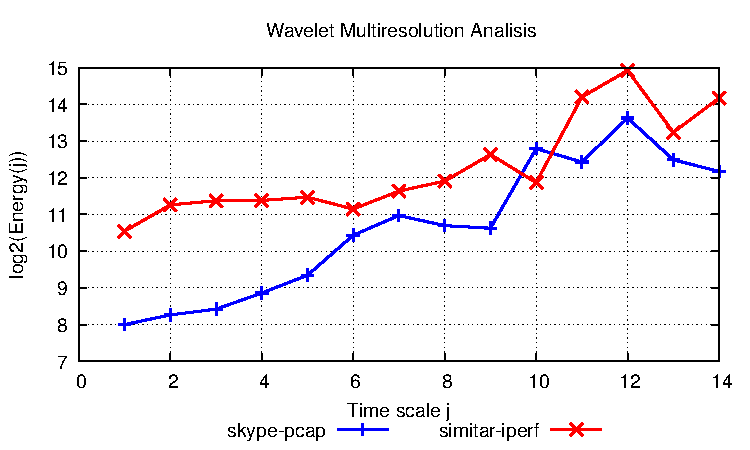
\includegraphics[width=77mm]{figures/skype-tree-iperf-WaveletMREA.pdf}
		\label{fig:iperftreeWaveletMREA}
	}
	\hspace{0mm}
	\subfloat[\textit{libtins, single-hop, skype-pcap}]{
		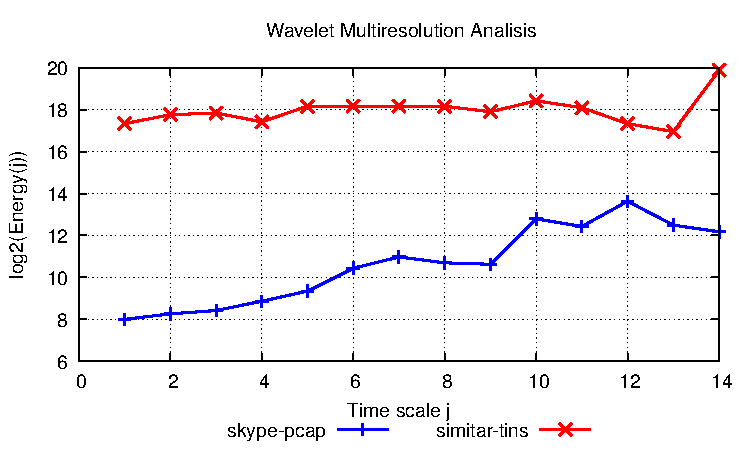
\includegraphics[width=77mm]{figures/skype-tins-WaveletMREA.pdf}
		\label{fig:tinsWaveletMREA}
	}
	\hspace{0mm}
		\subfloat[\textit{libtins, single-hop, langw10s-pcap}]{
			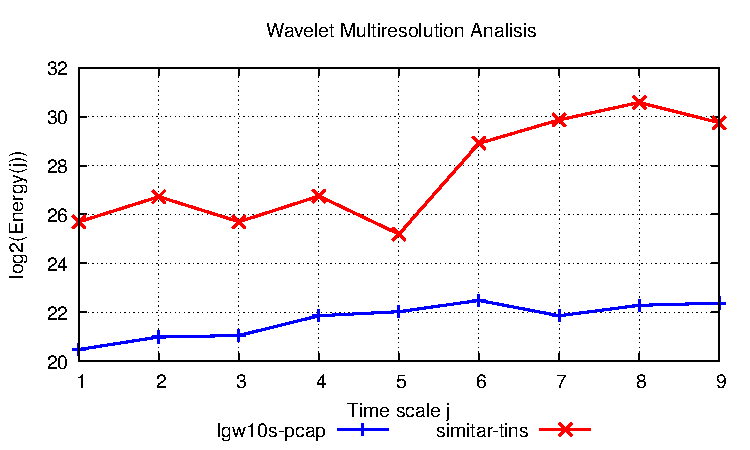
\includegraphics[width=77mm]{figures/lgw-tins-WaveletMREA.pdf}
			\label{fig:tinsLgwWaveletMREA}
		}
		\hspace{0mm}
	\caption{Wavelet multiresolution energy analysis.}
	\label{fig:wavelet}
\end{figure}


We display our results in the figures ~\ref{fig:flows-ps} to ~\ref{fig:wavelet}, and in the table ~\ref{tab:results-summary}, where the original and the synthetic traffics are compared. As we can see in the figure ~\ref{fig:flows-bandwidth}, the generated traffics are not identical regarding bandwidth, however both presents fractal-like shape. The Hurst exponent of inter-packet times in every case has an error smaller than 10\% compared to the original in every case. This result indicates that in fact, the fractal-level of each synthetic traffic is indeed similar to the original.  

The plot of flows per second seems much more accurate visually since most of the peaks match.  Indeed, no visual lag between the plots. We can analyze it precisely observing the cumulative flow distribution\ref{fig:flows-cdf}, where the results were almost identical on every plot. However, when SIMITAR is replicating the traffic of \textit{lgw10s-pcap} the number of flows per second decreases. It happens because of the methodology of traffic generation of the class \textit{TinsFlow} since it sends the packets of each stream as fast as possible. So each flow occurrence is restricted to smaller intervals. This behavior can be observed as well in the bandwidth plot. It is much larger in the first seconds and small at the end.

The best results achieved by SIMITAR were on the flow distribution characterization. On every experiment made, the cumulative distribution of flows was almost identical. The small imprecisions on the plots are expected and should result from threads and process concurrence of resources and imprecision on the sleep/wake signaling on the traffic generation side. Imprecisions on packet capture buffer may count as well since the operating system did the packet timing. This was our most significant achievement in our research. This result means that our method of flow scheduling and independent traffic generation were effective and efficient on replicating the original traffic at the flow-level. The actual number of flows was much more significant when SIMITAR used Iperf and about the same amount but little small when used libtins. This discrepancy happens with Iperf because it establishes additional connections to control the signaling and traffic statistics.  So, this more substantial number of flows comes from accounting, not just the traffic connections, but also with the signaling as well.  With libtins, the number of flows is small, because, if it fails to create a new traffic flow, this flows generation execution is aborted. 

On Wavelet multiresolution analysis of inter-packet times, the results have changed more in each case. The time resolution chosen was ten milliseconds, and it is represented in $\log_2$ scale. The actual time pf each time-scale $j$ value is given by the equation:

\begin{equation}
t = \frac{2^{j}}{100} [s]
\end{equation}

In the first case (figure ~\ref{fig:iperfWaveletMREA}), SIMITAR using Iperf in a single-hop scenario, on small time scales the energy level of the synthetic traffic remained almost constant, which indicates white-noise characteristics. The original skype traffic increased linearly, an indication of fractal shape. The synthetic trace started to increase at the time scale 5-6 (300-600 milliseconds). After this scale, the error between the curves become very small. One possible reason for this behavior is the fact that the constant which regulate the minimum burst time (\texttt{DataProcessor::m\_min\_on\_time}) is set to 100 milliseconds. For small time scales the traffic become similar to white noise since Iperf just emits traffic with constant bandwidth. For larger scales, it captures the same fractals patterns of the original trace. It also captures a periodicity pattern at the time-scale of 9 seconds. The authors of \cite{swing-paper} measured the same periodicity pattern. But on this trace, we observe some periodicity at 11 and 13 time-scales (20 and 80 seconds). 

In the second case, on a tree topology on small time scales, the same white-noise behavior is identified. We identify a similar behavior on the energy behavior on larger time-scales, but with a larger gap between the curves. Packet collision on switches requiring retransmission packets explains this behavior. In fact, as we can see in the table ~\ref{tab:results-summary}, two hundred more packets are leaving the client on the tree topology compared to the one-hop. 

On the last two plots, where we use libtins as packet crafter, the energy level is much higher, and the curves are much less correlated. SIMITAR are not modeling inter-packet with libtins, and are sending packets as fast as possible. We may observe on the figures ~\ref{fig:tinsBw} and ~\ref{fig:tinsLgwBw} that than have much  higher peaks compared to the original \textit{skype-pcap}.  As we see in the figure ~\ref{fig:tinsBw}, it just captured some periodicity characteristics at the time larger than 11-12 (20-40 seconds). SIMITAR determines larger periods between packets with session OFF times, and the session cut time (\texttt{DataProcessor::m\_session\_cut\_time}) is 30 seconds, that explain this behavior.


The current implementation still has problems on accurately reproduce \textit{pcaps} with high bandwidth values and a more substantial number of flows. The primary limitation is the time required to generate the trace descriptor.  The procedure is still mono-thread, and the linear regression procedure is not optimized. Although creating a trace descriptor of a small pcap file is fast, the time for processing large pcap file with thousands of flows is still prohibitively high, spending dozens of hours. 

Using the first 10 seconds of the trace \textit{bigFlows-pcap}, on 10 seconds of operation, Iperf generated much fewer packets than the expected. It is an expected behavior since the operating system couldn't handle so much newer processes (one per flow) in such short time. On the other hand, the same drawback wasn't observed using libtins as traffic generator tool, since being a low-level API makes it much computationally cheaper.  Some others unexpected behavior must have a more in-depth investigation, such as libtins generating more packets than expected for \textit{skype-pcap}, but not for \textit{lgw10s-pcap}, and why the creation of some flows fail, and how to fix it if possible. 

Another promising possible investigation is what traffic each tool can better represent. In terms of number of flows and packets, bandwidth and for larger \textit{pcaps}, \textit{libtins} is a best option. But Iperf has presented a better performance replicating scaling characteristics of applications. 

%%%%%%%%%%%%%%%%%%%%%%%%%%%%%%%%%%%%%%%%%%%%%%%%%%%%%%%%%%%%%%%%%%%%%%%%%%%%%%%%%%%%%%%%%%%%%%%%%%%%%%%%%%
\section{Conclusions}\label{sec:conclusion}


SIMITAR was designed to work at flow-level and packet level. At the flow-level, our methodology can achieve great results. In fact,  The cumulative distribution of flows is almost identical on each case. From the perspective of benchmark of a middle-box such as an SND switch, this is a great result, since its performance depends on the number of registered flows. However, because of packets exchanged by signaling connection, the traffic generated by Iperf, even following the same cumulative flow distribution, had created more streams then expected. 

At packet level, the current results with Iperf replicate with high accuracy the scaling characteristics of the original traffic, and the number of generated packets are not far than the expected. However, the packet size replication and therefore the bandwidth is not accurate. Also, \textit{libtins} as traffic generator tool still is limited in this aspect.

Once the current implementation of the Flow Generator still does not uses the whole set of parameters from the Compact Trace Descriptor, and many optimizations yet to be made, this is a satisfactory result that validates and proves the potential of our proposed methodology. Even we designing  SIMITAR  to prioritizing modularity over finner control, when we compare these current results with the more consolidated realistic traffic generator available, they are closer. At the flow-lever our results are at least as good as the achieved by Harpoon\cite{harpoon-paper} and Swing\cite{swing-paper}. At the scaling characteristics, on lightweight traces, they are already comparable in quality.




+++++++++++++++++++++++++++++++++

%%%%%%%%%%%%%%%%%%%%%%%%%%%%%%%%%%%%%%%%%%%%%%%%%%%%%%%%%%%%%%%%%%%%%%%%%%%%%%%%%%%%%%%%%%%%%%%%%%%%%%%%%%
\section{>>>>> Temp Introduction <<<<<< }\label{sec:introduction-temp}

On network benchmarking and testing, it is known that the traffic properties interfere on the network component performance\cite{burstiness-queue-lenght}\cite{harpoon-validation} and measurament acuracy\cite{swing-paper}. Studies show that a realistic Ethernet traffic provides a different and more variable load characteristics on routers\cite{harpoon-validation}, even with the same mean bandwidth consumption. A burstier traffic can cause packet more buffer overflows on network \cite{burstiness-queue-lenght} \cite{modelling-of-self-similar} \cite{empirical-interarrival-study}, degenerating network performance\footnote{Features such as packet-trains periods and inter-packet times affect traffic burstiness}. Also, a burstier and realistic traffic  impacts not just on performance, but on measurement accuracy as well \cite{legotg-paper} \cite{background-traffic-matter}. Along with that, buffers quees and software applications have performance degradation processing small-sized packets. All this indicates that tests with constant bit rate traffic generator tools such as Iperf and Ostinato are important but not enough to guarantee the SLAs for new technologies. 


Realistic workload generators are also essential security research\cite{ditg-paper}, and are crucial on the evaluation of firewall middleboxes. It includes studies of intrusion, anomaly detection, and malicious workloads\cite{ditg-paper}. Another critical point is the flow-oriented operation of SDN networks. Each new flow arriving on an SDN switch demands an extra communication load between it and the controller. This may create a bottleneck between the switch and the controller. We also have a flow-oriented operation on SDN switches. Since its operation relies on queries on flow tables, a stress load must have the same flow properties of an actual ISP scenario. 


Alongside with that the introduction of virtualization via techinologies such as NFV  still pose challenges on performance,  reliability, and security\cite{nfv-challenges}. Closed hardware solutions are easier to pass on Service Layer Agreement since they have a much more predictable behavior. We can expect that its impact mentioned before over virtualized middle-boxes should be even larger, due the extra overhead of a virtualization layer. Therefore, there is a demand for the study of the impact of a realistic traffic on this new sort of environment. How VNFs and virtualized middle-boxes and SDN testbeds will behave if stressed with a realistic traffic load in comparison to a constant rate traffic is a important subject on testing and benchmarking. 


The open-source community offers a huge variety of workload generators and benchmarking tools \cite{ditg-paper}\cite{validate-trafficgen}\cite{comparative-trafficgen-tools}\cite{performance-trafficgen}. Most of these tools were built for specific purposes and goals, so each uses different methods of traffic generation. Some traffic generator tools offer support emulation of single application workloads. But this does not correspond to real complex scenarios, with a large number of distributed hosts in an Internet Service Provider (ISP) or even a Local Area Network (LAN). Many tools support a larger set of protocols and high-performance, such Seagull and Ostinato. Others are also able to control inter-packet times and packet sizes using stochastic models, like D-ITG\cite{ditg-paper} and MoonGen. Since there is so many features and tools, selecting a good configuration is by itself a research project. How to use each parameter to simulate a specific scenario is a hard question \cite{legotg-paper}\cite{selfsimilar-ethernet}. It is a manual process and demands implementation of scripts or programs leveraging human (and scarce) expertise on network traffic patterns and experimental evaluation.



Some tools like Swing and Harpoon uses capture traces to set intern parameters, enabling an easier configuration. Also, Swing uses complex multi-levels models which are able to provide a high degree of realism\cite{swing-paper}. But they have their issues as well. Harpoon does not configure parameters at packet level\cite{harpoon-paper} and is not supported by newer Linux kernels, what may be a huge problem with setup and configuration. Swing\cite{swing-paper} aims to generate realistic background traffic, but do not reach high throughputs \cite{swing-paper} \cite{legotg-paper}. Due the fact that its traffic generation engine is coupled to its modeling framework, you can't opt to use a newer/faster packet generation library. The only way of replacing the traffic engine is changing and recompiling the original code. And this is a hard task.


Since synthetic traffic traces generation is mature in academia, the creation of custom network workloads through the configuration of high-throughput open-source is an affordable task. But it is not often available in an automatic way, and most of the times is a challenging question\cite{legotg-paper}, and still, requires expert knowledge. It requires time, study, and is vulnerable to human mistakes and lack of validation. Such work may require weeks to complete a realistic reproduction of a single scenario, so most of the time it is just not done. We argue that widely (i.e. affordable) existing approaches can be regarded as simplistic often point solutions to more general cases. 


Also, just choosing which workload generator tool may fit better for the user needs is not a simple question. Tools like D-ITG\footnote{\href{http://traffic.comics.unina.it/software/ITG/}{http://traffic.comics.unina.it/software/ITG/}} provide support to many different stochastic functions, Ostinato\footnote{\href{http://ostinato.org/}{http://ostinato.org/}} provides a larger support for protocols, and a higher throughput for each thread\cite{comparative-trafficgen-tools}, and others like Seagull\footnote{\href{http://gull.sourceforge.net/doc/WP_Seagull_Open_Source_tool_for_IMS_testing.pdf}{http://gull.sourceforge.net/doc/WP\_Seagull\_Open\_Source\_tool\_for\_IMS\_testing.pdf}} are responsive. 
















\addtolength{\textheight}{-12cm}   % This command serves to balance the column lengths
                                  % on the last page of the document manually. It shortens
                                  % the textheight of the last page by a suitable amount.
                                  % This command does not take effect until the next page
                                  % so it should come on the page before the last. Make
                                  % sure that you do not shorten the textheight too much.

\bibliographystyle{unsrt}

\bibliography{bibliography}

\end{document}
